\chapter{基于变长上下文的对话情绪识别}
\label{cha:erc}
本章专注于提升聊天机器人识别说话者情绪的能力,即对话情绪识别(Emotion Recognition in Conversation, ERC)。 现有的ERC方法使用固定的上下文窗口信息来识别说话者的情绪,这其中存在两个可能的问题:关键上下文信息的缺乏或冗余上下文信息的干扰,使得聊天机器人对说话者的判断不准确。本章探索如何利用可变上下文信息来解决以上两个问题。具体而言:~\ref{sec:erc_intro}节通过用具体的例子阐释以上两个问题来引出本章内容;~\ref{sec:erc_method}节详细描述了能够根据变长上下文信息来进行ERC的方法;然后~\ref{sec:erc_exp}节利用实验对提出的方法进行验证,最后~\ref{sec:erc_conclusion}节总结本章内容。
% 提出了一种更有效的 ERC 方法


% 作为回应,本章探讨了可变长度上下文的好处,并提出了一种更有效的 ERC 方法。在该方法中,在预测不同话语的情绪时利用不同的上下文窗口,并且包含两个新模块以实现可变长度上下文:1) 两个说话者感知单元,它显式地模拟说话者内部和说话者之间的依赖关系以提炼的对话上下文表示 2) 一个 top-k 规范化层,它确定最合适预测说话者情绪的对话上下文窗口。 实验和结果表明,该方法在三个公共数据集上优于几个强大的基线方法。

\section{引言}\label{sec:erc_intro}

对话中的情绪识别是根据先前的上下文和当前的话语来预测对话者在对话中的情绪的任务。演讲者的情绪是其心理状态的关键指标和影响因素。ERC的重大技术突破推动了医疗保健、消费品和金融服务等领域的应用发展~\cite{devillers2002annotation,nasukawa2003sentiment,forbes2004predicting,lee2005toward,devillers2006real,liu2012sentiment,poria2019emotion}。

\begin{figure}[ht]
\centering
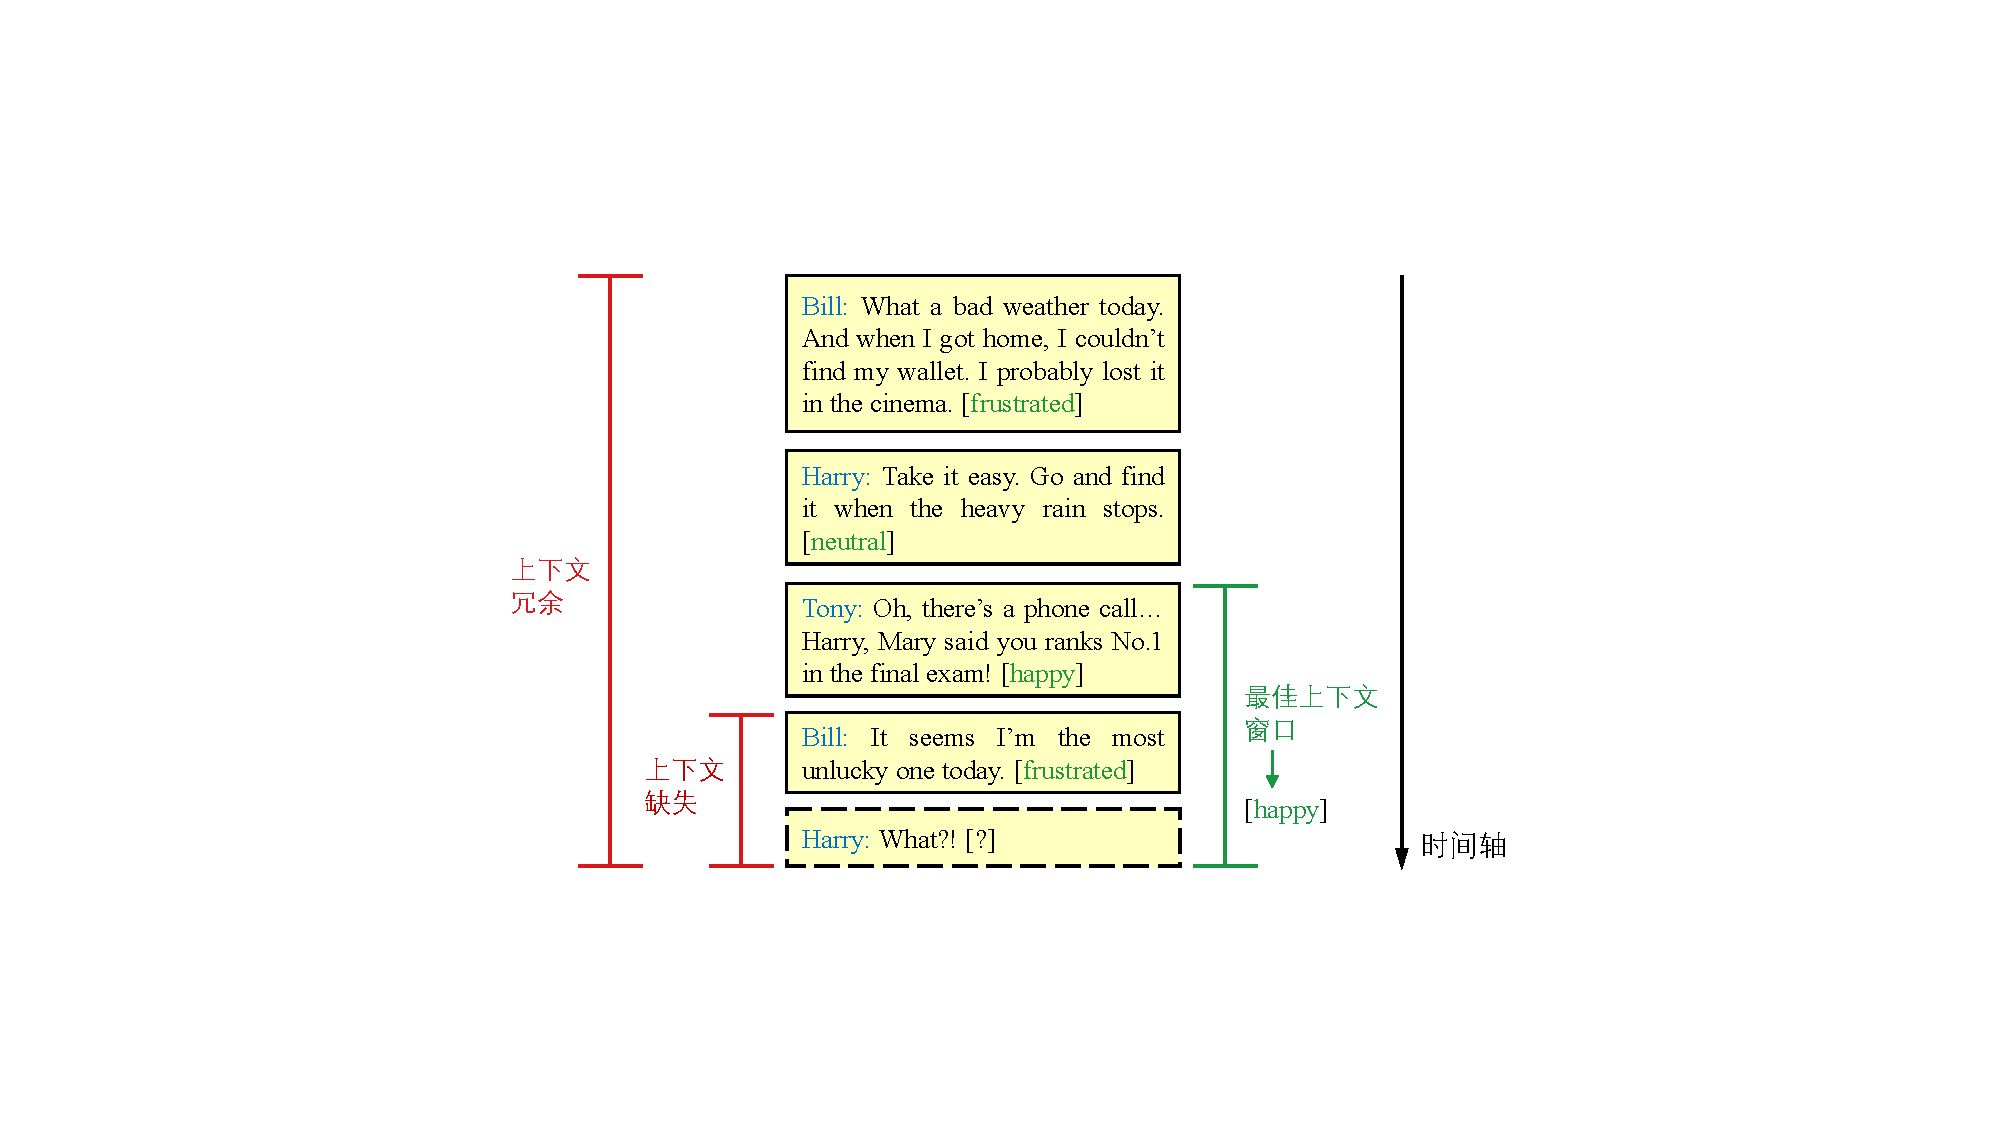
\includegraphics[width=0.7\textwidth]{erc_pics/example.pdf}
\caption{一个多方对话 ERC 示例。 \textit{Harry} 情绪的理想上下文窗口将恰好包括两个前面的话语,因为其中 \textit{Tony} 提供了 \textit{Harry} 快乐的证据。 \textit{Tony} 之前的话语是多余的,因为它们与当前的对话无关。}\label{fig:example}
\end{figure}

图 \ref{fig:example} 显示了 ERC 的一个示例。
现有方法~\cite{poria2017context,hazarika2018conversational,hazarika2018icon,majumder2019dialoguernn,ghosal2019dialoguegcn,ghosal2020cosmic,zhong2019knowledge,jiao2020real,jiao-etal-2019-higru}只考虑一个固定的上下文窗口(即前面的话语的数量),这可能会遇到两个问题:(1)上下文稀疏——由于窗口小而缺乏上下文; 或 (2) 上下文冗余——由于上下文窗口过大,包含来自不相关话语的冗余上下文。
例如,在图~\ref{fig:example} 中,正确预测当前话语(在虚线框中)的情绪需要至少两个先前的话语。 然而,包括任何更多的前面的话语是没有帮助的。因此,选择正确的上下文窗口对 ERC 至关重要。在这种情况下,知道当前说话者是 \textit{Harry} 有利于选择正确的上下文窗口,因为前面的话语之一明确提到\textit{Harry},表明它可能包含与当前话语相关的信息。也就是说,说话人依赖是确定正确上下文窗口的关键指标。

为了探索可变长度上下文的好处,本章提出了一种新的 ERC 方法:在对话中,话语之间的时序依赖和说话者依赖对于对话理解都至关重要~\cite{ghosal2020utterance},其中说话者依赖可以进一步分类为说话人内部和说话人之间的依赖关系~\cite{ishiwatari2020relation}。首先,通过一个基于注意力的话语编码器和两个说话者感知单元对上述依赖关系进行建模,以生成对话上下文表示,其中,内部和说话人之间的依赖关系被显式建模以帮助检测理想的上下文窗口。 接下来,一个top-k 归一化层基于降维后的上下文表示生成 top-k 最佳上下文窗口及其概率权重。最后,通过软性地利用 top-k 最佳上下文窗口来预测当前话语的情绪。

实验结果表明,该方法在三个公共对话数据集上取得了具有竞争力的性能:在两方对话数据集IEMOCAP~\cite{busso2008iemocap}和DailyDialog~\cite{li2017dailydialog}上分别得到了66.35\% 和61.22\%的F1,以及在多方对话数据集 EmoryNLP~\cite{zahiri2017emotion}上得到38.93\%的F1。广泛的消融研究证明了每个组件在该方法中的贡献以及使用可变长度上下文的必要性。

\section{方法}\label{sec:erc_method}
\subsection{任务定义}
一次对话由 $n$ 个按时间顺序排列的话语 $\{x_1, ..., x_t,...,x_n\}$ 及其说话者 $\{s_1, ..., s_t,...,s_n\}$ 组成。每个 $x_t$ 都是一个单词序列。 在时间步 $t$,ERC 的目标是在给定当前和之前的话语及其说话者的情况下,为说话者 $s_t$ 找出最可能的情感标签 $\hat{y}_t$:
\begin{equation}
    \hat{y}_t =\argmax p(y_t| x_{1:t}, s_{1:t}), \nonumber
\end{equation}
这里$x_{1:t}=\{x_1,...,x_{t}\}$并且$s_{1:t}=\{s_1,...,s_{t}\}$。

\subsection{方法}
如图 \ref{fig:overview} 所示,该方法由以下模块组成:
(1) 一种话语编码器,用于编码对话语之间的时序依赖;
(2) 两个说话人感知单元,明确编码说话人内部和说话人之间的依赖关系,以帮助检测理想的上下文窗口;
(3) 一个多层感知器和一个 top-k 归一化层,生成不同的上下文窗口的分布,从中确定 top-k 最佳上下文窗口及其相应的权重;
(4) 一个预测模块,它从具有不同概率权重的前 k 个最佳上下文窗口生成情绪分布。
\begin{figure}[ht]
\centering
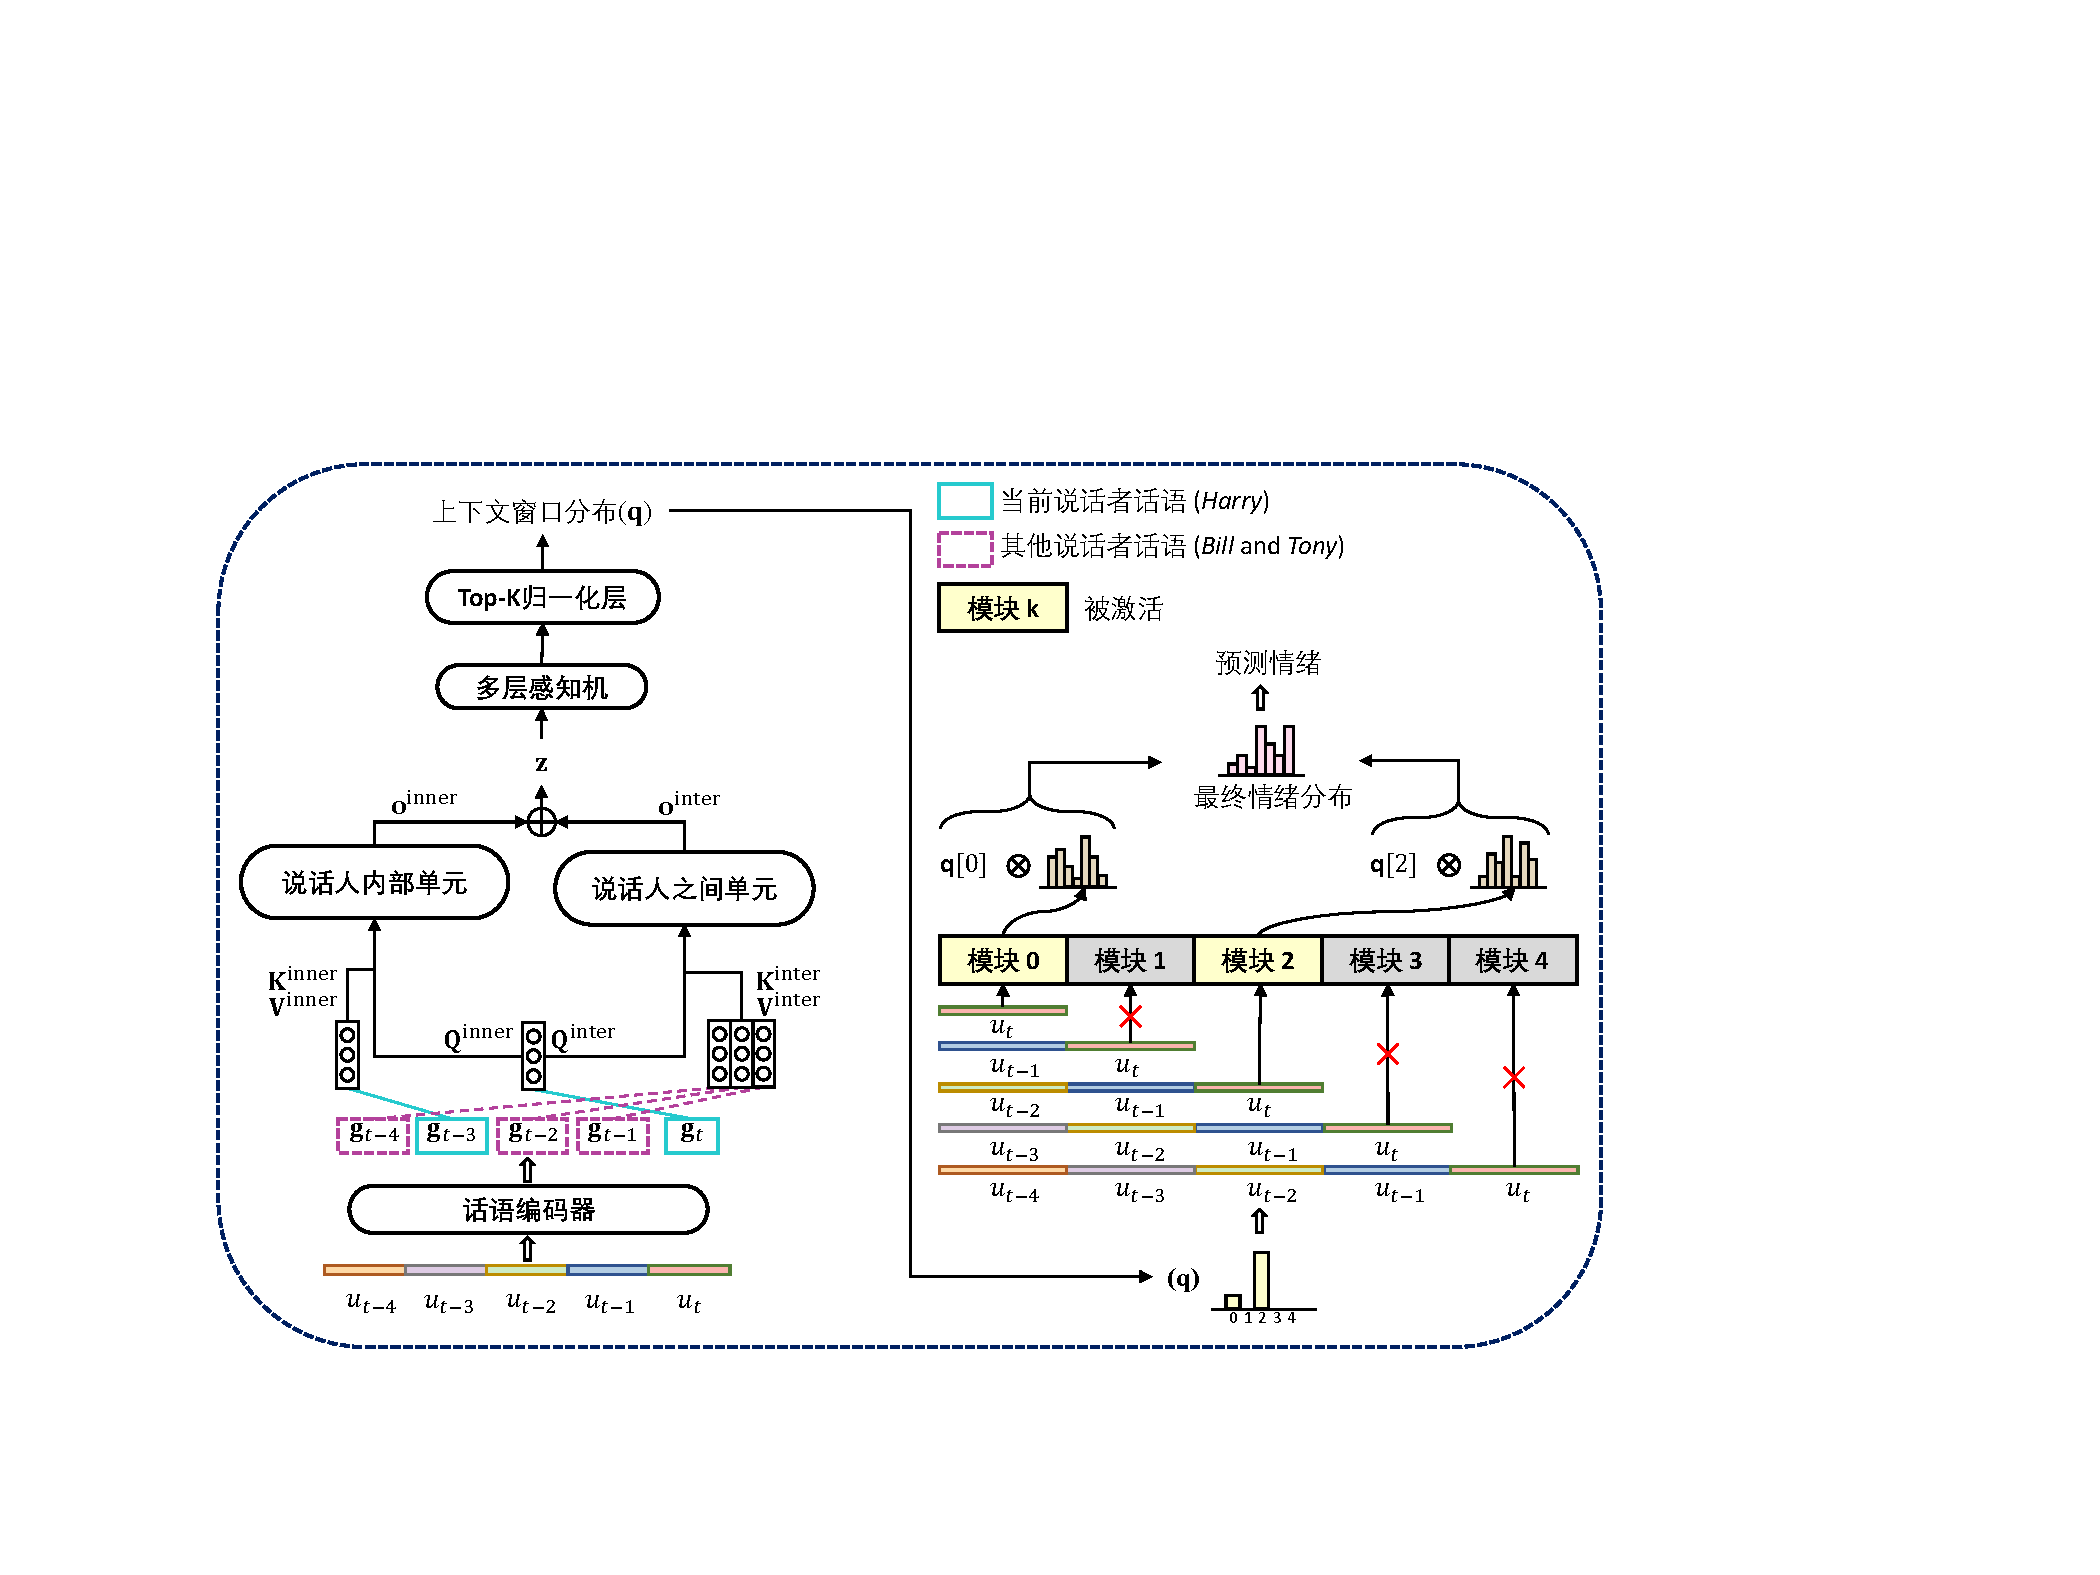
\includegraphics[width=\textwidth]{erc_pics/overview.pdf}
\caption{方法的总体架构。 图~\ref{fig:example} 中的实例用作输入。Step1:话语编码器对话语之间的时序依赖进行编码,并输出话语级表示。 第 2 步:说话人感知单元捕获说话人内部和说话人之间的依赖关系形成向量 $\mathbf{z}$。 Step3:上下文窗口分布 $\mathbf{q}$ 由 MLP 和 top-k 归一化层生成(这里使用 top-2 进行说明)。 Step4:以上下文窗口分布为条件进行情绪预测。 省略了特殊符号 \texttt{[CLS]}。}\label{fig:overview}
\end{figure}

\noindent\textbf{话语编码器 } 话语编码器的输入是一个带有说话人信息的符号序列。 在时间步 $t$,通过将说话人信息(即说话人的姓名)添加到每个话语之前生成输入序列,然后将直到时间步 $t$ 的话语连接成单个标记序列。 说话者的姓名和话语由特殊的 \texttt{[SEP]} 标记分隔。

输入序列被送入 RoBERTa~\cite{liu2019roberta} 的基础版本以编码话语之间的时序依赖并为每个话语生成上下文表示:
\begin{align}
    u_i &= s_i \oplus \texttt{[SEP]} \oplus x_i, \nonumber \\
    \left[\mathbf{g}_1, ...,\mathbf{g}_t\right] &= \textrm{RoBERTa}(\oplus_{i=1}^t u_i), \nonumber
\end{align}
其中 $\mathbf{g}_i$ 表示时间步长 $i$ 的话语的上下文表示,
对应于 $u_i$ 的第一个符号的 RoBERTa 输出。本章考虑最多 $M$ 个先前时间步长的上下文窗口,编码器输出向量序列 $\left[\mathbf{g}_{t-M}, ... , \mathbf{g}_t\right]$,其中 $\mathbf{g}_i \in \mathbb{R}^d$。

\noindent\textbf{说话者感知单位 } 本章提出的方法结合了说话人的依赖来指导理想上下文窗口的检测。
具体来说,提出的方法包含了两个说话人感知单元,来明确捕获说话人内部和说话人之间的依赖关系。这两个单元具有相同的基于注意力的结构,但它们不共享参数。首先将话语上下文表示 $\left[\mathbf{g}_{t-M}, ...,\mathbf{g}_{t-1}\right]$ 分成两个子集 $\mathbf{G}^\textrm{inner}$ 和 $\mathbf{G}^\textrm{inter}$,区分依据是它们对应的说话人是否与当前说话人相同。然后将相应的子集 $\mathbf{G}$ 和 $\mathbf{g}_t$ 输入对应的说话人感知单元,并应用多头注意力和层归一化~\cite{vaswani2017attention} 来合并说话人依赖:
\begin{align}
    \mathbf{o}&=\textrm{LayerNorm}(\mathbf{c} + \mathbf{g}_t), \nonumber \\
    \mathbf{c}&=\mathbf{W}^O \cdot \textrm{Concat}(\textrm{head}_1,...\textrm{head}_h), \nonumber \\
    \textrm{head}_i&=\textrm{Attention}(\mathbf{W}^Q_i\mathbf{g}_t, \mathbf{W}^K_i\mathbf{G}, \mathbf{W}^V_i\mathbf{G}), \nonumber
\end{align}
其中 $(\mathbf{W}^Q, \mathbf{W}^K, \mathbf{W}^V) \in \mathbb{R}^{d_k \times d}$ 和 $\mathbf{W}^ O \in \mathbb{R}^{d\times d}$ 是说话人特定的参数,$d_k = \frac{d}{h}$ 是每个注意力头的维度。注意力(Attention)定义同~\citet{vaswani2017attention}:
\begin{equation}
\textrm{Attention}(\mathbf{Q, K, V})=\mathbf{V} \cdot \softmax(\frac{\mathbf{K}^T\mathbf{Q}}{\sqrt{d_k}}). \nonumber
\end{equation}
接着将两个说话人感知单元的输出 $\mathbf{o}^\textrm{inner}$ 和 $\mathbf{o}^\textrm{inter}$ 拼接作为当前对话的上下文表示:
\begin{equation}\label{eq:z}
    \mathbf{z} = [\mathbf{o}^\textrm{inner};\mathbf{o}^\textrm{inter}] \in \mathbb{R}^{2d},
\end{equation}
$\mathbf{z}$编码了输入话语和说话者的信息以及它们的依赖关系。

\noindent\textbf{上下文窗口分布 } 接下来利用 $\mathbf{z}$ 生成 0 到 $M$ 上下文窗口对应的概率分布。具体而言是是通过以下方式完成的:(1) 一个多层感知器,它将$\mathbf{z}$映射到多个上下文窗口,以及 (2) 一个 top-k 归一化层,它在上下文窗口上生成分布。具体来说,首先将 $\mathbf{z}$ 送入一个双层 MLP 以获得上下文窗口的分数 $\mathbf{s}$:
\begin{align}
    \mathbf{h} &= \ReLU(\mathbf{W}_h\mathbf{z} + \mathbf{b}_h) \in \mathbb{R}^{d_h}, \nonumber \\
    \mathbf{s} &= \mathbf{W}_s\mathbf{h} + \mathbf{b}_s \in \mathbb{R}^{M+1}, \nonumber
\end{align}
其中 $\mathbf{W}_h \in \mathbb{R}^{d_h \times 2d}$, $\mathbf{W}_s \in \mathbb{R}^{(M+1) \times d_h}$ , $\mathbf{b}_h$ 和 $\mathbf{b}_s$ 是参数, $d_h$ 是隐藏层的维度。然后,根据$\mathbf{s}$中的值构造$\mathbf{s}$的top-$K$掩码,记为$\mathbf{m}$。如果 $\mathbf{s}[i]$ 在 $\mathbf{s}$ 中,$\mathbf{m}[i] = 0$ ,否则 $\mathbf{m}[i] = -\infty$,其中 $K$ 是一个超参数。 接着使用 $\softmax$ 对掩蔽的 $\mathbf{s}$ 进行归一化,以生成当前话语的上下文窗口分布$\mathbf{q}$:
\begin{equation}\label{eq:q}
    \mathbf{q} = \softmax(\mathbf{s} + \mathbf{m}) \in \mathbb{R}^{M+1}.
\end{equation}

\noindent\textbf{基于 top-$K$ 最佳上下文窗口的情绪预测 }
该方法没有使用 $\mathbf{q}$ 中概率最高的上下文窗口来预测情绪,而是使用 $\mathbf{q}$ 作为软标签,并在预测中利用所有 top-$K$ 上下文窗口。

如图 \ref{fig:overview} 所示,预测模块包含从 $0$ 到 $M$ 的 $M+1$ 个上下文模块 ,其中模块 $i$ 对应于上下文窗口 $i$ 的使用。
每个的输入,在其前面有一个 \texttt{[CLS]},由特定于模块的上下文编码器与话语编码器具有相同的架构。之后对 \texttt{[CLS]}, $\mathbf{g}^i_{\texttt{[CLS]}} \in \mathbb{R}^d$ 的编码器输出使用特定领域的线性分类器,以计算给定上下文窗口 $i$ 的情感标签分布 $\mathbf{p}^i$:
\begin{equation}
    \mathbf{p}^i = \softmax(\mathbf{W}^i\mathbf{g}^i_{\texttt{[CLS]}} + \mathbf{b}^i) \in \mathbb{R}^{c}, \nonumber
\end{equation}
其中 $\mathbf{W}^i \in \mathbb{R}^{c \times d}$ 和 $\mathbf{b}^i$ 是参数,$c$ 是情感类别的数量。

最终的情感标签分布 $\mathbf{\hat{p}}$ 结合了 top-$K$ 上下文窗口分布和给定不同上下文窗口的情感标签分布:
\begin{equation}\label{eq:p_hat}
    \mathbf{\hat{p}} = \sum_{i \in \textrm{top-}K}\mathbf{q}[i] \mathbf{p}^i \in \mathbb{R}^{c},
\end{equation}

\subsection{训练和预测}
对于训练,优化每个小批量对话样本 $\mathcal{B}$ 的交叉熵损失 $\mathcal{L}$:
\begin{equation}
    \mathcal{L} = \sum_{i=1}^{|\mathcal{B}|}\sum_{j=1}^{|\mathcal{B}_i|}-\log\;\mathbf{\hat{p}}^{ij}[y_{ij}], \nonumber
\end{equation}
其中 $|\mathcal{B}|$ 表示对话的数量, $|\mathcal{B}_i|$ 表示对话 $\mathcal{B}_i$ 中话语的数量, $y_{ij}$ 是 对话 $\mathcal{B}_i$ 和 $\mathbf{\hat{p}}^{ij}$ 中话语 $x_j$ 的黄金情感标签索引是相应的预测标签分布。

在测试时,根据等式 \ref{eq:p_hat} 中的最终情感标签分布 $\mathbf{\hat{p}}$ 选择情感标签 $\hat{y}$:
\begin{equation}
    \hat{y} = \argmax_i \mathbf{\hat{p}}[i]. \nonumber
\end{equation}

\section{实验}\label{sec:erc_exp}
\subsection{设置}
本章实验将新方法与经典方法DialogueRNN~\cite{majumder2019dialoguernn}、DialogueGCN~\cite{ghosal2019dialoguegcn}以及最新的方法RoBERTa-BASE~\cite{liu2019roberta}、KET~\cite{zhong2019knowledge}和COSMIC~\cite{ghosal2020cosmic} 在三个公开数据集进行了比较:两个双方对话数据集IEMOCAP~\cite{busso2008iemocap}、DailyDialog~\cite{li2017dailydialog} 和一个多方对话数据集 EmoryNLP~\cite{zahiri2017emotion}。这些数据集在对话者的数量、对话场景和情感标签上有所不同。 IEMOCAP~\cite{busso2008iemocap} 是一个多模态两方对话数据集,对话中的每个话语都用情绪标签\textit{argry}、\textit{sad}、\textit{happy}、\textit{excited}、\textit{frustrated} 或 \textit{neutral} 进行注释;DailyDialog~\cite{li2017dailydialog} 是一个单模态两方对话数据集,它涵盖了关于日常生活的各种主题,注释的情绪标签有\textit{anger}、\textit{disgust}、\textit{fear}、\textit{joy}、\textit{sadness}、\textit{surprise}和\textit{neutral};EmoryNLP~\cite{zahiri2017emotion} 是一个单模态多方对话数据集,它也是从 \textit{Friends}电视剧注释而来的,具有七个情绪标签:\textit{sad}、\textit{scared}、\textit{joyful}、\textit{mad}、\textit{powerful}、\textit{peaceful}和\textit{neutral}。实验中最多考虑 7 个($M=7$)之前的回合(即 8 个上下文模块)。上下文模块在数据集上进行了微调,并且它们的参数在训练期间被冻结。对于数据集 IEMOCAP、DailyDialog 和 EmoryNLP,各自的参数 $K=4,3,5$。 此外,对于说话人感知单元中的多头注意力,头的维度设置为 192,头数量设置为 4,dropout设置为 0.1。 对于说话人感知单元之后的 MLP,使用 256 的隐藏层大小。为了优化整个网络,实验中使用 AdamW 优化器~\cite{loshchilov2017decoupled} 和线性调度器来控制学习率的预热和衰减过程。具体来说,将预热比设置为 0.06,将峰值学习率设置为 2e-5,并将最大训练周期设置为 5。使用 32 的批量大小和 0.01 的 L2 权重衰减。 实验中根据开发集的性能选择超参数。 对于 DailyDialog,使用排除\textit{neutral}类的微平均F1 分数,\textit{neutral}类占整个数据集的百分比高达 83\%; 对于其他两个数据集,计算加权宏F1分数 ~\cite{zhong2019knowledge,ishiwatari2020relation}。 我们在五个随机种子下进行相同实验并报告平均结果。

\subsection{主要结果}
主要结果报告在表 \ref{tab:F1} 中。 我们提出的方法在数据集 IEMOCAP、DailyDialog 和 EmoryNLP 上达到了最佳性能,分别超过了最佳的基线方法COSMIC1.07\%、2.74\%和0.82\% F1 分数。该方法优于 COSMIC 的性能要归功于对可变长度上下文的考虑。 此外,与 COSMIC 不同,该方法不依赖于外部知识。 对于 IEMOCAP,我们的方法甚至在 F1 分数上以显著优势超过多模态模型 DialogueRNN,这表明 1)ERC 中的文本信息仍然需要更有效地利用,以及 2)该方法通过减轻上下文稀缺性来有效利用文本信息和上下文冗余问题。

\begin{table}[!ht]
\centering
\caption{主要结果。最好的 F1 分数以粗体突出显示。 - 表示未报告的结果。 CSK是commonsense knowledge(常识知识)的缩写。 $\star$ 表示实验中得到的结果。}
\label{tab:F1}
\small
\resizebox{0.65\textwidth}{!}{
\begin{tabular}{@{}lllll@{}}
\toprule
方法 & IEMOCAP & DailyDialog & EmoryNLP \\
\midrule
DialogueRNN \cite{majumder2019dialoguernn} & 62.75 & 50.65 & 31.70 \\
DialogueGCN \cite{ghosal2019dialoguegcn} & 64.18 & - & - \\
RoBERTa-BASE$^{\star}$ \cite{liu2019roberta} & 62.46 & 58.41 & 35.44 \\
KET \cite{zhong2019knowledge} & 59.56 & 53.37 & 34.39 \\
COSMIC \cite{ghosal2020cosmic} & 65.28 & 58.48 & 38.11 \\
COSMIC without CSK  & 63.05 & 56.16 & 37.10 \\
\midrule
Ours$^{\star}$ & \makecell[l]{\textbf{66.35}\\($\pm${0.21})} & \makecell[l]{\textbf{61.22}\\($\pm${0.16})} & \makecell[l]{\textbf{38.93}\\($\pm${0.23})} \\
\bottomrule
\end{tabular}
}
\end{table}

\subsection{消融实验}\label{sec:ablation}
为了揭示我们提出的方法中不同组件的贡献,我们对主要组件进行了消融实验:分别是说话人感知单元和上下文窗口分布的生成方法。

\noindent\textbf{说话人感知单元 } 将说话人感知单元与以下说话人依赖建模方法进行比较:
\begin{itemize}
    \item \textit{\textbf{N-Unit}}:\textit{N-Unit} 与说话人感知单元共享相同的结构。 与说话者感知单元不同的是,其输入的键和值都是先前的话语表示,而不管它们在说话者内部和说话者之间的关系。因此\textit{N-Unit} 是非说话人感知的。
    \item \textit{\textbf{S-Unit}}:\textit{S-Unit} 将指示每个话语的说话者的独热向量连接到话语表示,并执行与\textit{N-Unit}相同的操作。
    \item \textit{\textbf{GCNs}}:来自\citet{ghosal2019dialoguegcn}的方法,其中用多个图形卷积层捕获说话人的依赖。节点是话语,边权重是通过基于相似性的注意模块获得的。在其后添加一个最大池化层和一个线性层以获得向量 $\mathbf{z}$。\textit{GCNs} 的输入是话语编码器的输出。
\end{itemize}

表~\ref{tab:speaker}显示了比较结果。我们提出的方法优于 \textit{S-Unit} 的性能,因为我们的方法对说话人内部和说话人间依赖关系进行了显式建模。 \textit{S-Unit} 超过 \textit{N-Unit},表明说话人信息在 ERC 的上下文建模中不可或缺。
此外,说话人感知单元在二元数据集(IEMOCAP 和 DailyDialog)上的 F1 分数比其他三种方法中最好的方法高 0.33\% 和 0.72\%,低于多方数据集(EmoryNLP)上的 0.85\%. 这是因为多方对话中比二元对话更复杂的说话者依赖。当更多说话者参与对话时,我们的方法更善于捕捉说话者的依赖。
\begin{table}[ht!]
    \centering
    \caption{在测试集上说话人感知单元消融的结果。}
    \label{tab:speaker}
    \resizebox{0.55\textwidth}{!}{
    \begin{tabular}{llll}
        \toprule
        方法 & IEMOCAP & DailyDialog & EmoryNLP \\
        \textit{N-Unit} & 64.49 & 59.00 & 36.15 \\
        \textit{S-Unit} & 65.95 & 60.50 & 36.60 \\
        \textit{GCNs}  &  66.02 & 60.14 & 38.08 \\
        \midrule
        Ours  &  \textbf{66.35} & \textbf{61.22} & \textbf{38.93} \\
        \bottomrule
    \end{tabular}
    }
\end{table}

\noindent\textbf{上下文窗口分布的生成方法 } 上下文窗口分布$\mathbf{q}$(见等式\ref{eq:q})控制上下文模块的激活并作为注意力权重合并输出分布。 在我们的方法中,采用 MLP 和 top-k 归一化层来生成 $\mathbf{q}$。除此之外,尝试了 $\mathbf{q}$ 的其他几种生成方法,并将它们与我们的方法进行了比较。基于 $\mathbf{q}$ 的两个函数,上下文模块的 top-k 激活和输出分布加权,我们比较了以下的方法变体:
\begin{itemize}
    \item \textit{\textbf{All-Soft}}:我们方法中的 top-k 归一化层被 softmax 层替换以获得 $\mathbf{q}$,这意味着所有的 $M+1$ 上下文模块始终被激活,并且上下文字段的输出分布由注意力权重合并。
    \item \textit{\textbf{Topk-Hard}}:在top-k归一化层之后,$\mathbf{q}$中的$K$个非零概率被设置为$\frac{1}{K}$,也就是说 $K$ 激活的上下文模块的输出分布具有相同的权重。
    \item \textit{\textbf{All-Hard}}:不管时序和说话人的依赖如何,$\mathbf{q}$中的所有概率都设置为$\frac{1}{M+1}$,这意味着 所有 $M+1$ 上下文模块始终被激活,并且上下文模块的输出分布具有相同的权重。
    \item \textit{\textbf{Topk-Soft}}:我们提出的方法。
\end{itemize}

测试集的 F1 分数如表 \ref{tab:abla-select} 所示。 与 \textit{All-Hard} 相比,\textit{All-Soft} 仅在 EmoryNLP 上具有更好的性能。这是因为这样一个事实,即正确上下文窗口的注意力权重并不明显大于不正确上下文窗口的注意力权重。 因此,在我们的方法中直接禁用不正确的上下文字段比激活它们并给予它们较少的注意力权重更合理。 针对上述分析,\textit{Topk-Hard} 几乎在所有数据集中都优于 \textit{All-Hard},再次表明应该避免激活不正确的上下文字段。 top-k 归一化层提高了 $K$ 激活上下文字段的注意力权重,这表明 \textit{Topk-Soft} 优于 \textit{Topk-Hard}。
\begin{table}[ht]
\small
\centering
\caption{三个数据集测试集上上下文窗口分布生成方法的消融结果。}
\label{tab:abla-select}
\resizebox{0.55\textwidth}{!}{
\begin{tabular}{@{}lllll@{}}
\toprule
方法 & IEMOCAP & DailyDialog & EmoryNLP \\
\midrule
\textit{All-Soft} & 65.24 & 60.51 & 37.87 \\
\textit{Topk-Hard} & 65.75 & 60.22 & 38.23 \\
\textit{All-Hard} & 65.42 & 60.56 & 37.11 \\
\textit{Topk-Soft} & \textbf{66.35} & \textbf{61.22} & \textbf{38.93} \\
\bottomrule
\end{tabular}
}
\end{table}

\subsection{案例研究}
在表 \ref{tab:case} 中的第一个案例中,具有固定比较大的上下文窗口的 RoBERTa-BASE 产生错误答案 \textit{anger} 而考虑可变长度上下文的方法产生了正确的答案:\textit{Monica} 的情绪为 \textit{surprise}。 当 $K=2$ 时,我们的方法选择上下文窗口为0 和 1 进行情绪预测,阻止前两个话语中的冗余上下文。 在第二种情况下,具有固定上下文窗口为1的 RoBERTa-BASE 对 \textit{Rachel} 的情绪产生错误答案:\textit{sad},因为 RoBERTa-BASE 失去了关于 \textit{Racheal} 抱怨的关键上下文:前两句中哭泣的婴儿。并且,当$K=2$ 时,我们的方法认为最佳上下文窗口是 3 和 4,避免丢失关键上下文并产生正确答案 \textit{anger}。
\begin{table}[ht!]
\centering
\caption{来自 EmoryNLP 的测试实例。 比较了RoBERTa-BASE (RoB) 与新方法的结果。}
\label{tab:case}
\resizebox{0.6\textwidth}{!}{
\begin{tabular}{lp{5.5cm}ll}
\toprule
说话者 & 话语 & RoB & Ours \\
\midrule \midrule
\multicolumn{4}{l}{\textbf{样例1}}\\
\midrule
Chandler & Okay, is this lamp in the same place? & - & - \\
\midrule
Ross & Who cares? I repel women & - & - \\
\midrule
Chandler & No-no-no-no!!! You can‘t come in here! R-r-r-r-Ross is naked. & - & - \\
\midrule
Monica & What?! & \textcolor{dark-red}{anger} & \textcolor{dark-green}{surprise} \\
\midrule \midrule
\multicolumn{4}{l}{\textbf{样例2}}\\
\midrule
Rachel & Oh no just stopped to throw up a little bit. & - & - \\
\midrule
Rachel & Oh come on, what am I gonna do, its been hours and it won’t stop crying.  & - & - \\
\midrule
Monica & Umm, she Rach, not it, she. & - & - \\
\midrule
Rachel & Yeah, I’m not so sure.  & - & - \\
\midrule
Rachel & Oh my god, I am losing my mind.   & \textcolor{dark-red}{sad} & \textcolor{dark-green}{anger} \\
\bottomrule
\end{tabular}}
\end{table}


\section{本章小结}\label{sec:erc_conclusion}
为了缓解对话情绪分析中的上下文稀疏和上下文冗余问题,本章提出了一种新的对话情绪分析方法,能够从可变长度的上下文中识别说话者的情绪。精心设计的实验和消融研究证明了该方法的有效性。未来,我们倾向于通过外部知识或辅助任务来改进上下文窗口分布。此外,我们将继续探索检测适当上下文窗口的机制。
